
\documentclass[12pt]{article}
\usepackage[english]{babel}
\usepackage[utf8x]{inputenc}
\usepackage{amsmath}
\usepackage{graphicx}
\usepackage[colorinlistoftodos]{todonotes} 
\usepackage{xcolor}
\usepackage{listings}

\definecolor{mGreen}{rgb}{0,0.6,0}
\definecolor{mGray}{rgb}{0.5,0.5,0.5}
\definecolor{mPurple}{rgb}{0.58,0,0.82}
\definecolor{backgroundColour}{rgb}{0.95,0.95,0.92}

\lstdefinestyle{CStyle}{
    backgroundcolor=\color{backgroundColour},   
    commentstyle=\color{mGreen},
    keywordstyle=\color{magenta},
    numberstyle=\tiny\color{mGray},
    stringstyle=\color{mPurple},
    basicstyle=\footnotesize,
    breakatwhitespace=false,         
    breaklines=true,                 
    captionpos=b,                    
    keepspaces=true,                 
    numbers=left,                    
    numbersep=5pt,                  
    showspaces=false,                
    showstringspaces=false,
    showtabs=false,                  
    tabsize=2,
    language=C
}

\begin{document}

\begin{titlepage}

\newcommand{\HRule}{\rule{\linewidth}{0.5mm}} % Defines a new command for the horizontal lines, change thickness here

\center % Center everything on the page
 

\textsc{\LARGE Ecole Polytechnique Universitaire de Lille}\\[1.5cm] % Name of your university/college
\textsc{\Large Programmation Avancée}\\[0.5cm] % Major heading such as course name
\textsc{\large }\\[0.5cm] % Minor heading such as course title


\HRule \\[0.4cm]
{ \huge \bfseries Rapport Projet Correcteur Orthographique}\\[0.4cm] % Title of your document
\HRule \\[1.5cm]
 


\begin{minipage}{0.4\textwidth}
\begin{flushleft} \large
Corto \textsc{Callerisa} % Your name
\end{flushleft}
\end{minipage}
~
\begin{minipage}{0.4\textwidth}
\begin{flushright} \large
Sébastien \textsc{Dardenne} % Supervisor's Name
\end{flushright}
\end{minipage}\\[2cm]

% If you don't want a supervisor, uncomment the two lines below and remove the section above
%\Large \emph{Author:}\\
%John \textsc{Smith}\\[3cm] % Your name

%----------------------------------------------------------------------------------------
%	DATE SECTION
%----------------------------------------------------------------------------------------

{\large \today}\\[2cm] % Date, change the \today to a set date if you want to be precise

%----------------------------------------------------------------------------------------
%	LOGO SECTION
%----------------------------------------------------------------------------------------


\includegraphics[scale=0.4]{logo.png} % Include a department/university logo - this will require the graphicx package
 
%----------------------------------------------------------------------------------------
 
\vfill % Fill the rest of the page with whitespace

\end{titlepage}
\section{Introduction}
	

Ce projet a pour but d'appliquer les connaissances apprises lors du semestre 6 en programmation avancée. Il s'agit de réaliser un correcteur orthographique en utilisant un dictionnaire que l'on a préalablement chargé. De plus ce programme doit pouvoir extraire les mots d'un texte ou d'une liste afin de les vérifier.
\newline

\section{Principe}
Afin de minimiser l’espace mémoire nécessaire au stockage du dictionnaire tout en fournissant un temps de recherche bas, la structure de données que vous utiliserez sera un arbre préfixe (encore appelé trie). Il s’agit d’une structure arborescente pour laquelle des mots ayant des préfixes communs sont factorisés: chaque noeud de l’arbre est une lettre qui peut être terminale (i.e. dernière lettre d’un mot) ou pas.
\newline
\noindent
Considérons les mots: were et will. L’arbre (ou trie ) correspondant est affiché ci-dessous à gauche. Si on ajoute les mots we, wet et weave l’arbre est affiché à droite; les noeuds colorés représentant des lettres terminales.
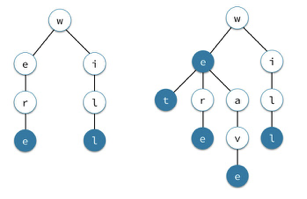
\includegraphics[scale=1.2]{arbre.png}
\newpage
\section{Structure de donnée}
	

\textit{Votre structure doit permettre de stocker et de manipuler un dictionnaire sous forme d'arbre préfixe / trie}
\newline
\newline
Pour la structure, nous avons eu deux idées principales, la première étant une structure sous forme de listes chainées néanmoins cette solution n'est pas optimale pour la recherche de caractère car la fonction parcours toute la liste dans le pire cas.

\newline
\noindent
Exemple avec les mots : cela, ces et cet:
\newline

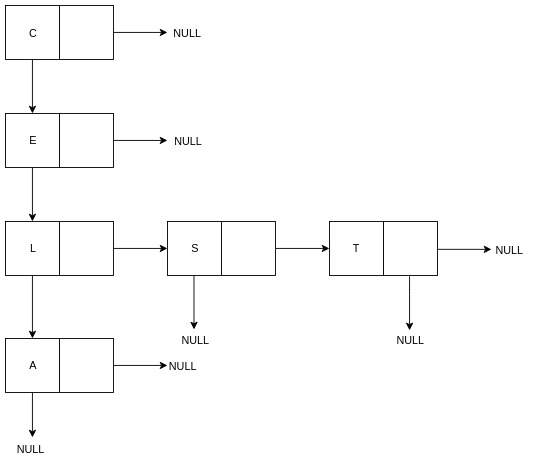
\includegraphics[scale=0.7]{structure1.jpeg}

\newpage

\newline
\noindent
Nous avons alors changé notre idée principale et donc nous avons choisit de partir sur une seconde solution qui est une structure avec un noeud composé de 26 pointeurs (un par lettre) et un booléen indiquant si le noeud fini un mot. Cette structure étant plus optimisé car elle s'actualise en fonction des lettres à ajouter en allouant la mémoire nécessaire.
\newline
\noindent
Exemple avec les mots : cela, ces et cet:
\newline

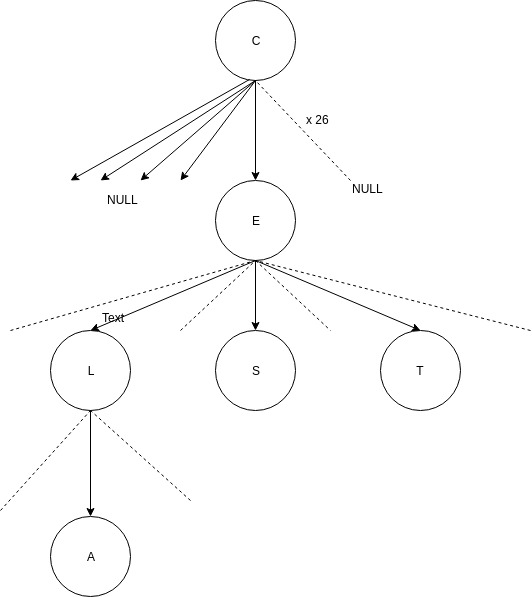
\includegraphics[scale=0.6]{structure2.jpeg}



\newpage

\section{Structure du programme}
\textit{Le programme permet de charger un dictionnaire à partir d'un fichier texte de données et analyse l'orthographe du fichier texte en indiquant les nombres de mots qui ne sont pas reconnus par le dictionnaire.}
\newline
\newline
Notre programme ce compose de 2 script principaux qui sont le dictionnaire et le correcteur, le dictionnaire permet d'importer un dictionnaire depuis un fichier texte et de vérifier l'appartenance d'un mot au dictionnaire importer. Le correcteur permet de vérifier l'orthographe de l'ensemble des mots d'un texte. Deplus, nous avons un MAKEFILE qui permet de compiler automatiquement les scripts.
\newline

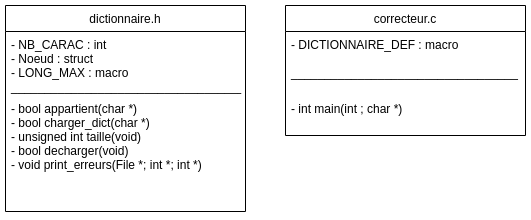
\includegraphics[scale=0.6]{structprg.png}


\newpage
\section{Respect du cahier des charges}

\underline{Cahier des charges:}
\begin{itemize}
\item Définir et implémenter une structure de données permettant de stocker et de manipuler un dictionnaire sous forme d’arbre préfixe / trie.
\item Charger un dictionnaire à partir d’un fichier texte de données. Ce fichier texte pouvant être un texte court, un roman ou une liste de mots.
\item Par exemple le fichier /etc/dictionaries-common/words est un dictionnaire de langue anglaise.
\item Analyser l’orthographe d’une phrase ou d’un texte en indiquant les nombres de mots qui ne sont pas reconnus par le dictionnaire.
\end{itemize}
\newline

\newline
\noindent
\underline{1. Structure de trie pour stocker et manipuler le dictionnaire :}
\noindent
\begin{lstlisting}[style=CStyle]
/*
   La structure principale du programme est un trie ou chaque Noeud possede jusqu'a 26 enfants ainsi qu'un booleen indiquant si le noeud termine un mot valide.
 */
typedef struct Noeud {
    bool mot_fini;
    struct Noeud *enfants[NB_CARAC];
} Noeud;
\end{lstlisting}
\newline
\newline 
\underline{2. Charger un dictionnaire  :}
\newline 
\noindent
Notre algorithme pour charger un dictionnaire est le suivant :
Après avoir chargé l'ensemble du fichier dictionnaire dans un buffer on rempli le trie caractère par caractère afin d'insérer les mots.
L'allocation de la mémoire permettant de charger le fichier est faite en une fois car l'on connait la taille en octets du fichier par l'appel à ftell() après avoir deplacé le pointeur de fichier à la fin.
Si un prefixe du mot courant a déja été importé on parcourt le chemin lorsque qu'il y a une déviation on initialises les noeuds correspondants.
L'apostrophe est gérée individuellement car son indice dans le tableau est un choix arbitraire.
Chaque fois que l'on recontre le caractère '\n', on l'absorbe et on boucle sur l'ajout du prochain mot.
\newline 
\noindent
La fonction importer\_dict() est contenue dans le fichier dictionnaire.c. Elle est commentée en détail.
\newline
\noindent
\underline{3. Détection d'erreurs :}
\newline
La détection des erreurs dans un texte est traitée dans le fichier correcteur.c qui fait des appels extensif à la fonction appartient() du fichier dictionnaire.c
L'algorithme est similaire à celui pour l'insertion :
On suit le parcours de l'arbre correspondant  au lettres du mot à verifier. Si chaque lettre correspond à un fils on renvoie la valeur du booléen mot\_fini du dernier noeud, et si le chemin entier n'existe pas on renvoie faux. Correcteur.c appel cette fonction pour chaque mot du dictionnaire traite les mots malorthographié en accord.


\section{Limites du projet et tests}
\newline
- Notre programme ne gère pas les mots avec accent et/ou caractère spéciaux. C'est pourquoi nous utilisons la langue anglaise pour les dictionnaires et les textes afin d'avoir que des lettres de l'alphabet et des apostrophes.

Le programme compile sans erreurs et reporte pas de fuites mémoire en utilisant l'utilitaire valgrind.
\end{document}